\documentclass[tikz,border=5pt]{standalone}
\usepackage{fontspec}
\setmainfont{Times New Roman}
\usepackage{unicode-math}
\setmathfont{Cambria Math}
\usetikzlibrary{shapes.geometric,positioning,fit,backgrounds,arrows.meta,calc}

\begin{document}
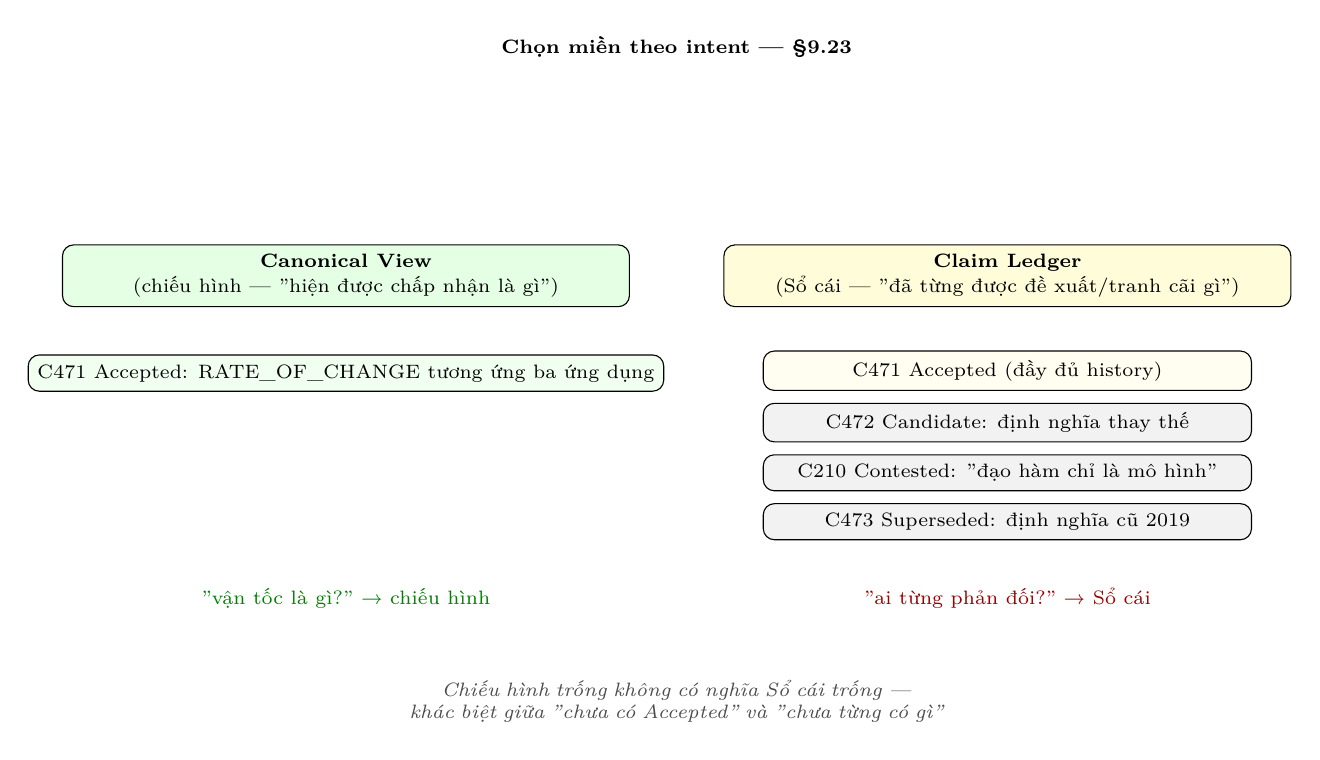
\begin{tikzpicture}[
  box/.style={rectangle, draw, rounded corners, align=center, minimum width=7.2cm, font=\scriptsize},
  claim/.style={rectangle, draw, rounded corners, fill=gray!10, align=center, minimum width=6.2cm, font=\scriptsize},
  arrow/.style={-{Stealth[length=2.2mm]}, thick},
  label/.style={font=\scriptsize\itshape, text=gray!60!black},
]

% === Canonical view ===
\node[box, fill=green!10] (canon) at (-4.2, 2.2) {\textbf{Canonical View} \\[1pt] (chiếu hình — "hiện được chấp nhận là gì")};
\node[claim, below=0.6cm of canon, fill=green!6] (c1) {C471 Accepted: RATE\_OF\_CHANGE tương ứng ba ứng dụng};

% === Ledger ===
\node[box, fill=yellow!15] (ledg) at (4.2, 2.2) {\textbf{Claim Ledger} \\[1pt] (Sổ cái — "đã từng được đề xuất/tranh cãi gì")};
\node[claim, below=0.55cm of ledg, fill=yellow!6] (g1) {C471 Accepted (đầy đủ history)};
\node[claim, below=0.15cm of g1] (g2) {C472 Candidate: định nghĩa thay thế};
\node[claim, below=0.15cm of g2] (g3) {C210 Contested: "đạo hàm chỉ là mô hình"};
\node[claim, below=0.15cm of g3] (g4) {C473 Superseded: định nghĩa cũ 2019};

% === Question routing ===
\node[font=\scriptsize, align=center] at (0, 5.1) {\textbf{Chọn miền theo intent — §9.23}};

\node[font=\scriptsize, align=center, text=green!50!black] at (-4.2, -1.9)
  {"vận tốc là gì?" → chiếu hình};

\node[font=\scriptsize, align=center, text=red!60!black] at (4.2, -1.9)
  {"ai từng phản đối?" → Sổ cái};

\node[font=\scriptsize\itshape, text=gray!60!black, align=center, text width=11cm] at (0, -3.2)
  {Chiếu hình trống không có nghĩa Sổ cái trống —\\khác biệt giữa "chưa có Accepted" và "chưa từng có gì"};

\end{tikzpicture}
\end{document}